\subsection{Performance comparisons}
As can be seen on \autoref{tab:results-with-many-methods} LightGCN outperforms all the other methods by a significant amount.
With our dataset NGCF performs better than PUP by a small amount, even though Price-Aware recommendation in their paper showcased the opposite \cite{Priceaware}.
Price-Aware recommendation also used a Yelp dataset from 2018 for their experiments, while our Yelp dataset is from 2020 and therefore is a bit larger than theirs.
The results also showcase, that there is a large decrease in performance, when adding prices and categories to the adjacency matrix in LightGCN, which makes it perform worse than any of other baseline methods.
For NGCF PAS the same changes in input only makes it differentiate negatively by a small amount and actually still performs better than PUP.
\begin{table*}[h!]
    \centering
    \begin{tabular}{|l|l|l|l|l|}
        \hline
        \rowcolor[HTML]{FFFFFF}
                       & \multicolumn{4}{l|}{\cellcolor[HTML]{FFFFFF}Yelp Dataset}                                                       \\ \hline
        Method         & Recall@50                                                 & NDCG@50         & Recall@100      & NDCG@100        \\ \hline
        LightGCN       & \textbf{0.2106}                                           & \textbf{0.1063} & \textbf{0.3176} & \textbf{0.1344} \\ \hline
        PUP            & 0.1697                                                    & 0.07802         & 0.2654          & 0.1023          \\ \hline
        GCN            & 0.1558                                                    & 0.07593         & 0.2442          & 0.1001          \\ \hline
        NGCF           & 0.1810                                                    & 0.08817         & 0.2769          & 0.1132          \\ \hline
        GCMC           & 0.1692                                                    & 0.0835          & 0.2497          & 0.1008          \\ \hline
        LGCN PAS (1.0) & 0.1542                                                    & 0.0717          & 0.2199          & 0.086           \\ \hline
        NGCF PAS (1.0) & 0.1749                                                    & 0.0849          & 0.2743          & 0.1111          \\ \hline
    \end{tabular}
    \caption{Results for the experiment with the different methods}
    \label{tab:results-with-many-methods}
\end{table*}
The recall@50 and NDCG@50 for NGCF, NGCF PAS, LightGCN and LGCN PAS can be seen on \autoref{fig:ndcg-50k-lgcn-ngcf-ngcfpas-pas} and \autoref{fig:recall-50k-lgcn-ngcf-ngcfpas-pas}.
Recall@100 and NCDG@100 for the same methods can be seen on \autoref{fig:ndcg-100k-lgcn-ngcf-ngcfpas-pas} and \autoref{fig:recall-100k-lgcn-ngcf-ngcfpas-pas}.
The figures show that there is not a big difference between the NGCF and NGCF PAS graphs and that NGCF outperforms NGCF PAS by 3.48\% in Recall\@50, 1.04 in NDCG\@50, 1.01 in Recall\@100 and 1.02\% in NDCG\@100.
However for LightGCN and LGCN Pas, there is a large difference.
LGCN PAS has a large decrease in performance, and the graph fluctuates a lot, and does not improve when training.
In fact LGCN performs better by 36.6\% in Recall\@50, 48.3 in NDCG\@50, 44.4\% in Recall\@100 and 56.3\% in NDCG\@100.
\begin{figure}
    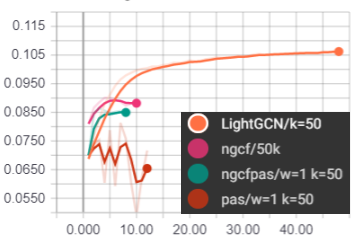
\includegraphics[width=\linewidth]{figures/graphs/ndcg-50k-lgcn-ngcf-ngcfpas-pas.png}
    \caption{NDCG$@$50k on LightGCN, NGCF, NGCF PAS and PAS.}
    \label{fig:ndcg-50k-lgcn-ngcf-ngcfpas-pas}
\end{figure}

\begin{figure}
    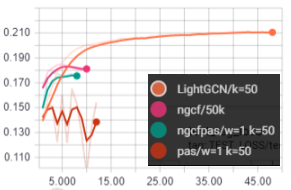
\includegraphics[width=\linewidth]{figures/graphs/recall-50k-lgcn-ngcf-ngcfpas-pas.png}
    \caption{Recall$@$50k on LightGCN, NGCF, NGCF PAS and PAS}
    \label{fig:recall-50k-lgcn-ngcf-ngcfpas-pas}
\end{figure}

\begin{figure}
    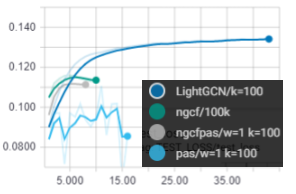
\includegraphics[width=\linewidth]{figures/graphs/ndcg-100k-lgcn-ngcf-ngcfpas-pas.png}
    \caption{NDCG$@$100k on LightGCN, NGCF, NGCF PAS and PAS.}
    \label{fig:ndcg-100k-lgcn-ngcf-ngcfpas-pas}
\end{figure}

\begin{figure}
    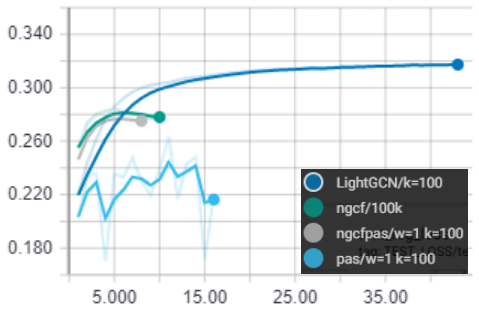
\includegraphics[width=\linewidth]{figures/graphs/recall-100k-lgcn-ngcf-ngcfpas-pas.png}
    \caption{Recall$@$100k on LightGCN, NGCF, NGCF PAS and PAS.}
    \label{fig:recall-100k-lgcn-ngcf-ngcfpas-pas}
\end{figure}


\subsubsection{Hyperparameter experiment}
As described in \autoref{subsec:simple-extension}, we utilize a hyperparameter that is inserted into the adjacency matrix, whenever there is a connection between the item nodes and category nodes, or item nodes and price nodes.
Experiments are done with the hyperparameter $X$ in LGCN PAS and NGCF PAS with the values $0.0$, $0.5$, $1.0$ and $2.0$ to see what effect this has on the performance.
\begin{table*}[h!]
    \centering
    \begin{tabular}{|l|l|l|l|l|}
        \hline
        \rowcolor[HTML]{FFFFFF}
                       & \multicolumn{4}{l|}{\cellcolor[HTML]{FFFFFF}Yelp Dataset}                                   \\ \hline
        Method         & Recall@50                                                 & NDCG@50 & Recall@100 & NDCG@100 \\ \hline
        LGCN PAS (0.0) & 0.1560                                                    & 0.07674 & 0.2456     & 0.09901  \\ \hline
        LGCN PAS (0.5) & 0.1591                                                    & 0.07825 & 0.2539     & 0.1010   \\ \hline
        LGCN PAS (1.0) & 0.1542                                                    & 0.0717  & 0.2199     & 0.086    \\ \hline
        LGCN PAS (2.0) & 0.1526                                                    & 0.07573 & 0.1581     & 0.06509  \\ \hline
        NGCF PAS (0.0) & 0.1758                                                    & 0.08483 & 0.2737     & 0.1111   \\ \hline
        NGCF PAS (0.5) & 0.1756                                                    & 0.08472 & 0.2744     & 0.1108   \\ \hline
        NGCF PAS (1.0) & 0.1749                                                    & 0.08485 & 0.2743     & 0.1111   \\ \hline
        NGCF PAS (2.0) & 0.1741                                                    & 0.08371 & 0.2762     & 0.1116   \\ \hline
    \end{tabular}
    \caption{Results for the experiment using different input values.}
    \label{tab:hyperparameter-results}
\end{table*}
As can be seen in \autoref{tab:hyperparameter-results} inserting categories and price into the adjacency matrix decreases the performance compared to LightGCN.
The best performing $X$ value is 0.5, followed by 0.0 according to our tests.
Giving prices and categories the same or higher input value as the connection between item and user therefore decreases the performance.
On \autoref{fig:ndcg-pas-weights} and \autoref{fig:recall-pas-weights} it can be seen that the graphs fluctuate with the input values that were used.
There could be multiple reasons for this generally not performing well.
The embeddings created from this input could be used, so that it tries to recommend prices and categories, which is not possible.
Another reason could be because LightGCN does not utilize feature transformation and the nonlinear activation function.
LightGCN performs well, if there are only user and item ids, and the decrease in performance could be because LightGCN is unable to handle the semantic representations of price and category.\\
For NGCF changing the input value of price and categories changes almost nothing.
This can also be seen on \autoref{fig:ndcg-pas-weights} and \autoref{fig:recall-ngcfpas-weights}.
This is likely because the embeddings for price and categories are never used.
However, we did have an initial idea, that the convolutions with price and category would be reflected onto users and items, which is seen to give a very minimal effect on the outcome.


\begin{figure}
    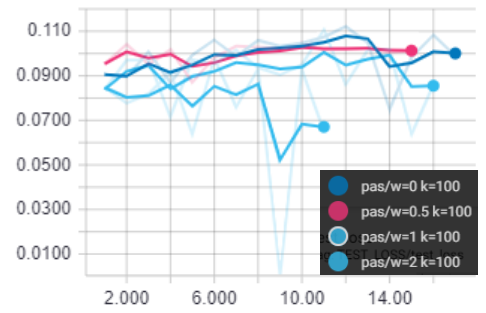
\includegraphics[width=\linewidth]{figures/graphs/ndcg-pas-weights.png}
    \caption{NDCG$@$100 on PAS with different input values}
    \label{fig:ndcg-pas-weights}
\end{figure}

\begin{figure}
    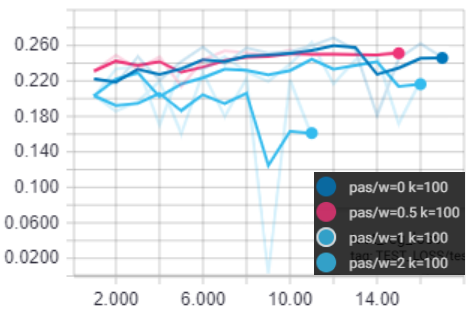
\includegraphics[width=\linewidth]{figures/graphs/recall-pas-weights.png}
    \caption{Recall$@$100k on PAS with different input values}
    \label{fig:recall-pas-weights}
\end{figure}

\begin{figure}
    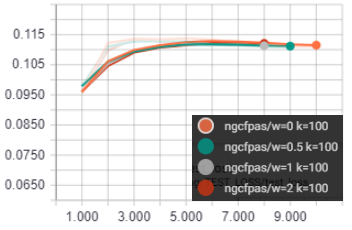
\includegraphics[width=\linewidth]{figures/graphs/ndcg100-ngcfpas-weights.png}
    \caption{NDCG$@$100k on NGCF PAS with different input values}
    \label{fig:ndcg-ngcfpas-weights}
\end{figure}

\begin{figure}
    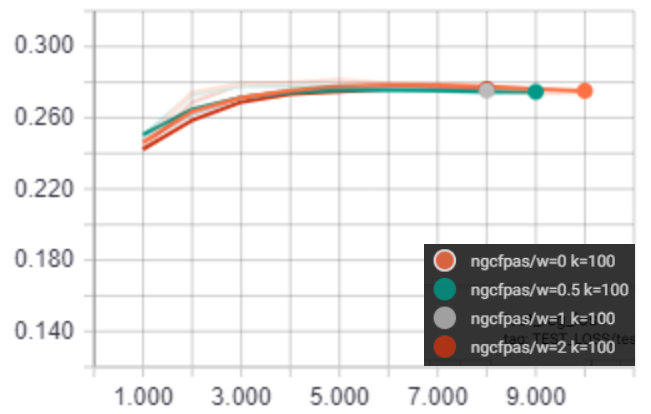
\includegraphics[width=\linewidth]{figures/graphs/recall-ngcfpas-weights.png}
    \caption{Recall$@$100k on NGCF PAS with different input values}
    \label{fig:recall-ngcfpas-weights}
\end{figure}

\subsubsection{Experiment with one convolution}
An experiment was conducted to see what influence it would have on the performance of the methods to change the number of convolutions to one.
The results from this experiment can be seen in \autoref{tab:one-convolution}.
When comparing the results with the previous experiment in \autoref{tab:results-with-many-methods} that used 3 convolutions for all methods except PUP, it can be seen that NGCF and LightGCN have a worse performance when evaluating them with Recall@50 and NDCG@50.
However for NGCF PAS it can be seen that the number of convolutions have little influence on the results.
Its performance decreased with 0.0001 in Recall@50 and improved with 0.00082 in NDCG@50.
LGCN PAS performs significantly worse, which can be seen on \autoref{fig:one-con-ndcg} and \autoref{fig:one-con-recall}.
LGCN PAS actually performs worse as it trains when only using one convolution.
This experiment shows that the benefit of convolutions depends a lot on what method is used.
Methods such as NGCF PAS and LGCN PAS do not get a large benefit from the additional convolutions, but for LightGCN and NGCF the additional convolutions improve their performance.
\begin{table}[]
    \centering
    \begin{tabular}{|l|l|l|}
        \hline
        \rowcolor[HTML]{FFFFFF}
                       & Recall@50 & NDCG@50 \\ \hline
        LightGCN       & 0.1953    & 0.0957  \\ \hline
        PUP            & 0.1697    & 0.07802 \\ \hline
        NGCF           & 0.1748    & 0.08422 \\ \hline
        LGCN PAS (1.0) & 0.1299    & 0.06454 \\ \hline
        NGCF PAS (1.0) & 0.1748    & 0.08572 \\ \hline
    \end{tabular}
    \caption{Results for experiment with one convolution}
    \label{tab:one-convolution}
\end{table}

\begin{figure}
    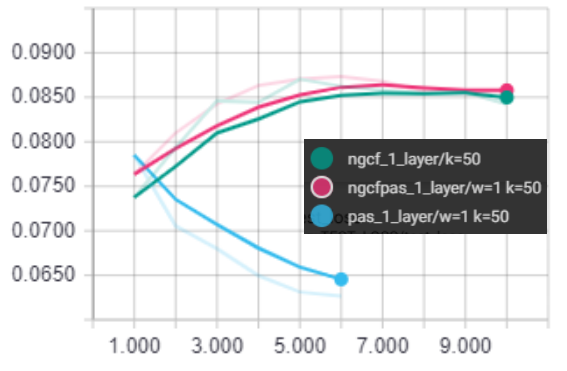
\includegraphics[width=\linewidth]{figures/graphs/one-convolution-ndcg.png}
    \caption{NDCG$@$50k with one convolution}
    \label{fig:one-con-ndcg}
\end{figure}

\begin{figure}
    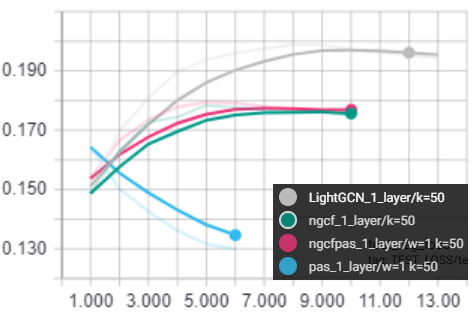
\includegraphics[width=\linewidth]{figures/graphs/one-convolution-recall.png}
    \caption{Recall$@$50k with one convolution}
    \label{fig:one-con-recall}
\end{figure}
